\section{theory}\label{sec:theory}
In this section we will present the main contribution of the paper:
First we present the abstract syntax of the programs that the analysis is defined for, further we define the conversion from program to program graph and give the abstract syntax for instructions appearing on the edges within such graphs.
Next we formalize the abstract semantics, and thereafter we argue, through several proof sketches, that the abstract semantics are sound.
At last we prove that our analysis will always terminate.

\subsection{Abstract Syntax} \label{subsec:function-definitions}
% Casper says: The reader should know what abstract syntax is...
% This section will introduce the syntactic sets and abstract syntax of SQAAL.
% The syntactic sets of SQAAL encompass the various elements and constructs that constitute the language's grammar.
% These sets define the valid combinations of symbols and keywords that form syntactically correct statements in SQAAL. They include components such as keywords, identifiers, operators, literals, and punctuation marks, each serving a specific role in expressing queries and analytical operations.

This paper adopts a modified version of the abstract syntax originally presented in~\cite{cortesi_abstract_2013}.
Omitted parts within this simplified abstract syntax correspond to features or constructs that are not utilized or discussed in the context of the current application.
Certain constructs have been modified to enhance clarity, most notably:
\begin{itemize}
    \item variables representing database names $v_d \in \mathbb{V}_d$ has been introduced.
    \item Database variables from \cite{halder_abstract_2012} are now called column variables, in symbols $v_t \in \mathbb{V}_t$.
\end{itemize}

The abstract syntax of SQAAL is defined in terms of the syntactic sets introduced in \autoref{tab:syntatic-sets}.
\begin{figure}[htb!]
     \center
    \begin{tabular}{r p{0.65\columnwidth }}
    $n \in \mathbb{Z}$                          & Integers                                                   \\
    $k \in \mathbb{S}$                                  & Strings                                                    \\
    $c \in \mathbb{C}$                          & Constants                                                 \\
    $v_a \in \mathbb{V}_a$                      & Application variables                                     \\
    $v_d \in \mathbb{V}_d$                      & Database variables \\
    $v_t \in \mathbb{V}_t$                    & Column variables   \\
    $v \in \mathbb{V} = \mathbb{V}_a \cup \mathbb{V}_t$ & Variables                                                 \\
    $e \in \mathbb{E}$                          & Arithmetic expressions                                    \\
    $b \in \mathbb{B}$                          & Boolean expressions                                       \\
    $\tau \in \mathbb{T}$                       & Terms                                                     \\
    $a_f \in \mathbb{A}_f$                      & Atomic formulas                                           \\
    $\phi  \in \mathbb{W}$                      & Well-formed formulas (pre-condition part of SQL commands) \\
    $A_{sql} \in \mathbb{A}_{sql}$              & Action part of SQL commands                               \\
    $C_{sql} \in \mathbb{C}_{sql}$              & SQL commands                                              \\
    $I \in \mathbb{I}$                          & Instructions/commands                                     \\
    \end{tabular}
    \caption{Syntatic Sets}
    \label{tab:syntatic-sets}
\end{figure}

The abstract syntax of SQAAL is presented in \autoref{tab:abstract-syntax}.
For simplicity's sake we assume that $\mathbb{V}_a$, $\mathbb{V}_d$ and $\mathbb{V}_t$ are mutually disjoint.

\begin{figure}[htb!]
    \center
    \begin{tabular}{r p{0.65\columnwidth}}
        $c ::=$ & $n \mid k$ \\
        $v ::=$ & $v_t \mid v_a$ \\
        $e ::=$ & $c \mid v \mid op_u\; e \mid \;e_1 op_b\; e_2$ for $op_u = \{-, lower, upper, bit\_lenght lenght\}$ and $op_b = \{+, -, *, /, ||\}$ \\

        $b ::=$ & $e_1 = e_2 \mid e_1 \leq e_2 \mid e_1 < e_2 \mid \neg b \mid b_1 \lor b_2 \mid b_1 \land b_2 \mid \texttt{true} \mid \texttt{false}$ \\

        $a_f ::=$ & $e_1 = e_2 \mid e_1 \leq e_2 \mid e_1 < e_2$ \\
        $\phi ::=$ & $a_f \mid \neg \phi_1 \mid \phi_1 \lor \phi_2 \mid \phi_1 \land \phi_2 \mid \forall v_n \phi \mid \exists v_n \phi$ \\
        $A_{sql} :: =$ & $select(v_a, v_d, \mathbf{v}_t) \mid update(v_d, \mathbf{v}_t, \mathbf{e}) \mid delete(v_d) \mid insert(v_d, \mathbf{v}_t, \mathbf{e})$ \\
        $C_{sql} ::=$ & $\langle A_{sql}, \phi \rangle $ \\
        $I ::=$ & $skip \mid v_a := e \mid v_a := ? \mid C_{sql} \mid b$ \\
    \end{tabular}
    \caption{Abstract Syntax}
    \label{tab:abstract-syntax}
\end{figure}

\subsection{Abstract Domains}\label{subsec:abstract-domains}

In the following section we will describe the abstract domains of our value analysis.

\subsubsection{Abstract domain of strings as regular expressions}\label{subsubsec:abstract_domains_strings}
We have chosen regular expressions/languages to represent the abstract domain of the family of SQL string data types.
Regular expressions/languages are chosen instead of more powerful representations because of the decidable nature of inclusion and equality between them.

Let $\regexs$ denote the set of regular expressions, for elements of $\regex \in \regexs$ we denote the language of $\regex$ as $\lang(\regex)$.
In general we will not distinguish between $R$ and $\lang(\regex)$ when it simplifies matters.
The lattice of $(\regexs, \subseteq, \cup, \cap)$ is a lattice but not a finite one, this is a problem: Essentially, we want the state-space our analysis to be finite, such that we can employ the Kleene fixed-point theorem (see \autoref{thm:kleene_finite}) to prove the termination of our analysis.
If the state-space is built from infinite parts the state-space itself will be infinite.
We will 'fix' this problem later in \autoref{sec:cover-lattice}.
Naturally we define the concretisation of regular expression as it's language:
\begin{align}
    \concrete_6 &: \mathbf{REG} \rightarrow \mathcal{P}(\mathbf{STR}) \\
    \concrete_6(R) &= \mathcal{L}(R)
\end{align}
Where $\strs$ denote the set of all strings.

\subsubsection{Abstract domain of integers as union intervals}\label{subsubsec:abstract_domains_numbers} We have chosen a finite union and intersection of intervals to represent the abstract domain of the family of SQL number data types.
We call them union of intervals as all such objects can be written as a union of intervals.
We only consider integers, but we imagine that the domain can be easily extended to the reals.
Let $\mathbf{INT}$ be the set of union intervals, that is inductively defined as:
\[
    \inference{i \text{ is an interval}}{i \in \mathbf{INT}} \quad
    \inference{\mathscr{I}_1 \in \textbf{INT} & \mathscr{I}_2 \in \textbf{INT}}{\mathscr{I}_1 \cup  \mathscr{I}_2 \in \mathbf{INT}} \quad
    \inference{\mathscr{I}_1 \in \textbf{INT} & \mathscr{I}_2 \in \textbf{INT}}{\mathscr{I}_1 \cap  \mathscr{I}_2 \in \mathbf{INT}}
\]

For integers we will only consider $[a, b], [a, +\infty)$ and $(-\infty, b]$ where $a, b \in \mathbb{Z}$ as valid intervals.

This abstract representation of numbers $(\uints, \subseteq, \cup, \cap)$ has the same issue as regular expressions: It is not finite.
We define the concretisation of union intervals as follows:
\begin{align}
    \concrete_6 &: \mathbf{INT} \rightarrow \mathcal{P}(\mathbf{NUM}) \\
    \concrete_6(\uint_1 \cup \uint_2) &= \concrete_6(\uint_1) \cup \concrete_6(\uint_2) \\
    \concrete_6(\uint_1 \cap \uint_2) &= \concrete_6(\uint_1) \cap \concrete_6(\uint_2) \\
    \concrete_6([a, b]) &= \left\{ z \in \mathbb{Z} \middle| a \leq z \leq b \right\} \\
    \concrete_6([a, +\infty]) &= \left\{ z \in \mathbb{Z} \middle| a \leq z \right\} \\
    \concrete_6([-\infty, b]) &= \left\{ z \in \mathbb{Z} \middle| z \leq b \right\}
\end{align}

This abstract domain is most likely not a new development, the title of \cite{li2010abstract} suggest a similar construct, but we have been unable to get a hold of their paper.

\subsubsection{Cover lattice}\label{sec:cover-lattice}
To resolve the issues presented above, we introduce the notion of a cover lattice.
As above the idea presented here is probably not novel.
Before we can define a cover lattice, we need to define the notion of a top-cover.

\begin{definition}
    A finite non-empty subset $X \subseteq S$ of a lattice $(S, \subseteq, \cup, \cap)$ is called a collectively top-cover of $S$ whenever $\bigcup X = \top$.
\end{definition}

\begin{definition}\label{def:coverlattice}
Given a collectively top-cover $X$ of a lattice $(S, \subseteq, \cup, \cap)$.
A cover lattice of $S$ in respect to $X$ denoted $\clattice{X}{S}$ is the minimum set where,
For $X$ and $S$:
\begin{align}
    \inference{x \in X}{x \in C_X(S)} \quad
    \inference{x_1 \in C_X(S) & x_2 \in C_X(S)}{x_1 \cup  x_2 \in C_X(S)} \quad
    \inference{x_1 \in C_X(S) & x_2 \in C_X(S)}{x_1 \cap  x_2 \in C_X(S)}
\end{align}
\end{definition}

As a note when we use the notation $C_X(S)$ we always assume that $X$ is a top cover of $S$.
The notion of a cover lattices gives rise to the following theorem:

\begin{restatable}{theorem}{partition}\label{thm:partition}
For a non-complete lattice $(S, \subseteq, \cup, \cap)$ and collectively top-cover $X$ of $S$, the cover lattice $(\clattice{X}{S}, \subseteq, \cup, \cap)$ is a finite and complete lattice.
\end{restatable}

And the following lemmas immediately follow:

\begin{lemma}
    If $\mathcal{R}$ is a top-cover of $(\regexs, \subseteq, \cup, \cap)$ then $(\clattice{\mathcal{R}}{\regexs}, \subseteq, \cup, \cap)$ is a finite and complete lattice.
\end{lemma}

\begin{lemma}
    If $\mathcal{I}$ is a top-cover of $(\uints, \subseteq, \cup, \cap)$ then $(\clattice{\mathcal{I}}{\uints}, \subseteq, \cup, \cap)$ is a finite and complete lattice.
\end{lemma}

We now define the function that maps an elements in a lattice to the most precise element in a corresponding cover lattice:
\begin{align}
    \cdot \into C_X(S) &: S\rightarrow C_X(S) \\
    s \into C_X(S) &= \bigcap\{s' \in C_X(S)|s \subseteq s'\}
\end{align}
We overload this notation to work on sets of values in particular for $S' \subseteq S$ we define:
\begin{align}
    \cdot \into C_X(S) &: \mathcal{P}(S) \rightarrow \mathcal{P}(C_X(S)) \\
    S' \into C_X (S) &= \{s \into C_X(S) \mid s \in S'\}
\end{align}


% \begin{definition}
%     We define $\cdot \into C_X(S):S\rightarrow C_X(S)$ to be the function mapping $s\in S$ to the least element in $C_X(S)$ containing it, that is $s \into C_X(S)=\bigsqcap\{s'\in C_X(S)|s\sqsubseteq s'\}$
%     \\
%
%     We define $\cdot \into C_X(S):\mathcal{P}(S)\rightarrow \mathcal{P}(C_X(S))$ to be the function that maps the powerset$(\mathcal{P})$ of the lattice elements to the powerset of the cover lattice elements$(C_X (S))$.
%     We use $H \into C_X (S) = \{h \into C_X (S) \mid h \in H\}$ to show how a set of elements$(H)$ is mapped to the cover lattice.
% \end{definition}

% todo I don't think the definition below is ever used, uncomment it if you find a case
% \begin{definition}
%     We define $\cdot \into C_\mathcal{X}(\mathcal{S}): \bigtimes_{i = 1}^{n} S_i \rightarrow \bigtimes_{i = 1}^{n} C_{X_i}(S_i)$ to be the function that takes a tuple and inserts each element of the tuple correctly into its given cover lattice.
%     We use $(h_1, h_2 \dots h_n)\into C_{\mathcal{X}}(\mathcal{S})=(h_1 \into C_{X_1}(S_1), h_2\into C_{X_2}(S_2), \dots, h_n \into C_{X_n}(S_n))$, where $\mathcal{X}=(X_1, X_2, \dots, X_n)$ and $\mathcal{S}=(S_1, S_2, \dots, S_n)$ to show how a tuples elements are inserted into the cover lattice what $\mathcal{X}$ and $\mathcal{S}$ are.
% \end{definition}

\begin{example}
    \autoref{fig:tikz-reg-partition} illustrates a simple lattice cover of the regular languages.
    The regular language $R$ is represented by the gray circle and its complement $\overline{R}$ is represented by the white circle.
    The union of the two regular language represent the entire regular language $\Sigma^*$ and their intersection is the empty set $\emptyset$.

    \autoref{fig:tikz-reg-partition-lattice} illustrates the cover lattice induced by the lattice cover.
    The top element $\top$ is the entire regular language $\Sigma^*$ and the bottom element $\bot$ is the empty set $\emptyset$.
\end{example}

% Tikzfigures
\begin{figure}
    \center
    \resizebox{7.5cm}{!}{
    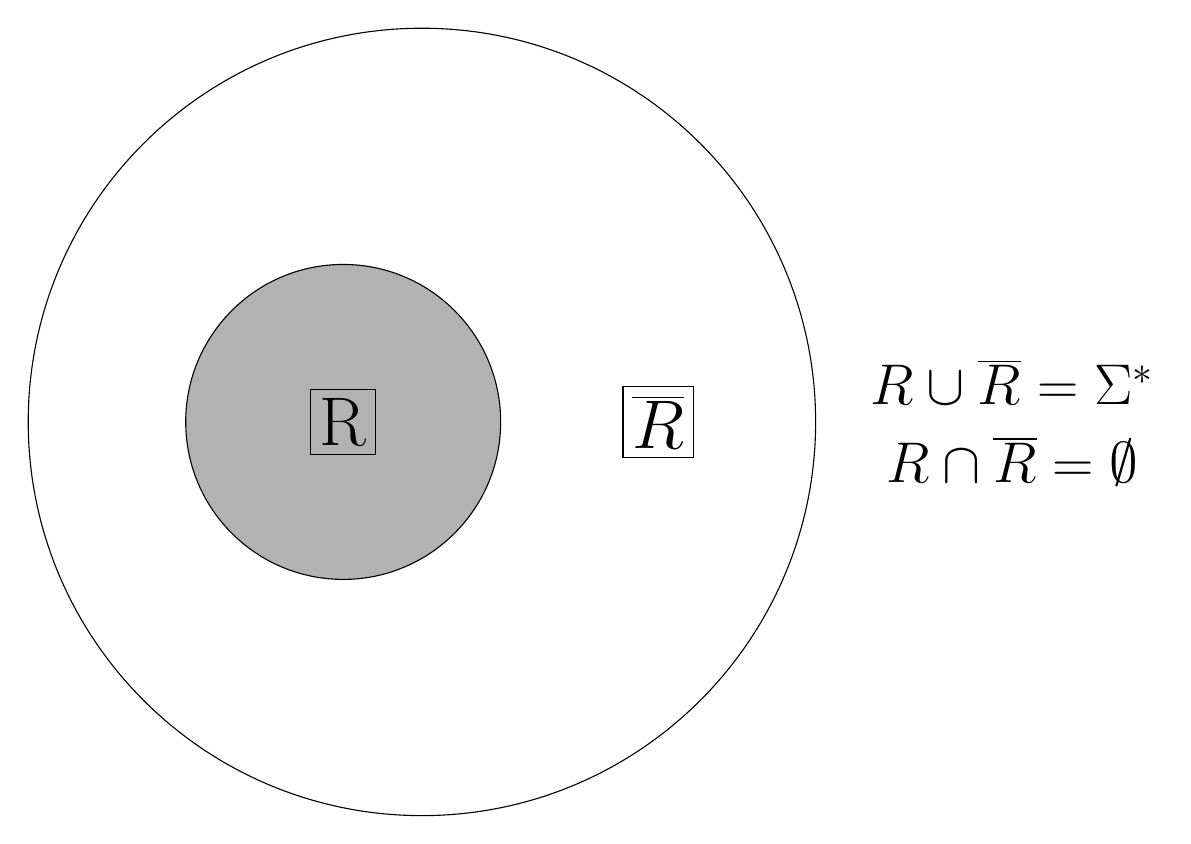
\begin{tikzpicture}
    \filldraw[fill=white, draw=black] (2,2) circle (5cm);
    \node [draw] at (5,2) {\Huge$\overline{R}$};
    \filldraw[fill=gray!60, draw=black] (1,2) circle (2cm);
    \node [draw] at (1,2) {\Huge R};
    \node at (9.5, 2.5) {\huge $R \cup \overline{R} = \Sigma^*$};
    \node at (9.5, 1.5) {\huge $R \cap \overline{R} = \emptyset$};
\end{tikzpicture}}
    \caption{Regular language partition}
    \label{fig:tikz-reg-partition}
\end{figure}

\begin{figure}[!htb]
    \center
    \resizebox{6.5cm}{!}{
    \begin{tikzpicture}
    \usetikzlibrary{calc}
    \node (a) [state] {$R \cup \overline{R} = \top = \Sigma^*$};
    \node (b1) [state, shift={($(a.south)+(1cm, -1cm)$)}] { $R$};
    \node (b2) [state, shift={($(a.south)+(-1cm, -1cm)$)}]{ $\overline{R}$};
    \node (c) [state, shift= {($(a.south) + (0cm, -2.5cm)$)}] { $R \cap \overline{R} = \bot = \emptyset$};
    \draw (a) to (b1);
    \draw (a) to (b2);
    \draw (b1) to (c);
    \draw (b2) to (c);
\end{tikzpicture}}
    \caption{Regular language partition as a lattice}
    \label{fig:tikz-reg-partition-lattice}
\end{figure}

\subsubsection{Abstract tuples}

We define abstract tuples as the product lattice of $\regexs$ and $\uints$ intertwined depending on the schema of the table.
And we define the concretisation function as follows:
\begin{align}
    \concrete_5 &: \bigtimes_{i = 1}^{n}(S_i) \rightarrow \mathcal{P}\left(\bigtimes_{i = 1}^n Z_i \right) \\
    \concrete_5(\ab{e_1}, \ab{e_2}, \dots, \ab{e_n}) &= \concrete_6(\ab{e_1}) \times \concrete_6(\ab{e_2}) \times \dots \times \concrete_6(\ab{e_n})
\end{align}
Where $S_i$ either is $\regexs$ or $\uints$ and $Z_i$ is correspondingly $\strs$ or $\mathbf{NUM}$.

\subsubsection{Single and List values}
When we consider the abstract domain of strings and numbers, we need to consider both single values and lists of values.
We would like to distinguish between single values and lists of values, thus for some set $S$ we define the set $\mathsf{Val} \; S$ inductively as:
\begin{align}
    \inference{}{\bot \in \mathsf{Val} \; S} \quad
    \inference{s \in S}{\mathsf{Single} \; s \in \mathsf{Val} \; S} \quad
    \inference{S' \subseteq S}{\mathsf{List} \; S' \in \mathsf{Val} \; S} \quad
\end{align}
We can define the lattice, $(\mathsf{Val} \; A, \subseteq, \cup, \cap)$, we first define the relation of the lattice:
\begin{align}
    \mathsf{Single} \; s &\sqsubseteq \mathsf{List} \; S \quad
    \text{iff} \; s \in S \\
    \mathsf{Single} \; s_1 &\sqsubseteq \mathsf{Single} \; s_2 \quad
    \text{iff} \; s_1 \sqsubseteq s_2 \\
    \mathsf{List} \; S &\not\sqsubseteq \mathsf{Single} \; s\\
    \mathsf{List} \; S_1 &\sqsubseteq \mathsf{List} \; S_2 \quad
    \text{iff} \; \forall s_1 \in S_1, \; \exists s_2 \in S_2: \; s_1 \sqsubseteq s_2\\
\end{align}

    We define $\cdot \into C_X(S): \ \mathsf{Val} \ S \rightarrow \mathsf{Val} \ C_X(S)$ to be the function that takes some value and inserts it into its cover lattice. \\
    For single elements we use $(\mathsf{Single} \ h) \into C_X(S) = \mathsf{Single}(h\into C_X(S)) \\$
    we say $x \in (\mathsf{Single} \ x') \ \text{iff} \ x = x'.$ \\
    And for a list of elements, we use $(\mathsf{List} \ H) \into C_X(S)=\mathsf{List}(H\into C_X(S))\\$
    we say $x \in (\mathsf{List} \ X) \ \text{iff} \ x \in X.$

We can define the joins and meets of the lattice as follows:
\begin{align}
    \mathsf{Single} \; s \sqcup \mathsf{List} \; S &= \mathsf{List} \; (S\sqcup\left\{ s \right\})\\
    \mathsf{Single} \; s_1 \sqcup \mathsf{Single} \; s_2 &= \mathsf{Single} \; (s \sqcup s )\\
    \mathsf{List} \; S_1 \sqcup \mathsf{List} \; S_2 &= \mathsf{List} \; (S_1 \sqcup S_2)\\
    \mathsf{Single} \; s \sqcap \mathsf{List} \; S &= \mathsf{Single} \; s\\
    \mathsf{List} \; S_1 \sqcap \mathsf{List} \; S_2 &= \mathsf{List} \; (S_1 \sqcap S_2)\\
    \mathsf{Single} \; s_1 \sqcap \mathsf{Single} \; s_2 &= \mathsf{Single} \; (s_1 \sqcap s_2)\\
    \mathsf{List} \ \emptyset \sqcap \mathsf{Single} \ s &= \ \perp
\end{align}
We see that if a list is empty and we look for the meet with a single value, it is equivalent to $\perp$.
As the lattice $(\mathsf{Val} \; A, \subseteq, \cup, \cap)$ is finite, we can use the Kleene fixed-point theorem (see \autoref{thm:kleene_finite}) to prove the termination of our analysis.

We define the concretisation of a variable value as:
\begin{align}
    \concrete_{4a} &: \mathsf{Val} \; \left(C_{X}(S)\right) \rightarrow \mathcal{P}(Z \cup Z^\star) \\
    \concrete_{4a}(\mathsf{Single} \; \ab{s}) &= \concrete_6(\ab{s}) \\
    \concrete_{4a}(\mathsf{List} \; \ab{S'}) &= \bigcup_{n \in \mathbb{N}}\left\{s_1, s_2, \dots, s_n \in Z^n \middle| \forall i \in \{1, 2, \dots, n\} : \exists \ab{s} \in \ab{S'} : s_i \in \concrete_6(\ab{s}) \right\}
\end{align}


\subsubsection{Abstract domain of tables}\label{subsubsec:abstract_domain_of_tables}

We consider a table $t$ as function from the domain of possible tuples in the table $\mathbb{T}$ to the codomain of natural numbers including $0$, $\mathbb{N}$:
\begin{equation}
    t : \mathbb{T} \rightarrow \mathbb{N}.
\end{equation}
The function $t$ describes the number of a given tuple in a table.
We can then consider abstraction over the table $t$ by abstracting either the domain or codomain.
This gives rise to a taxonomy of abstract domains of tables shown in \autoref{tab:taxonomy_of_abstract_domain_of_tables}.
In \autoref{tab:taxonomy_of_abstract_domain_of_tables}, $\mathbb{T}^\#$ denotes an abstract domain of the set of possible tuples $\mathbb{T}$, such that it forms a finite lattice $(\mathbb{T}^\#, \sqsubseteq, \sqcap, \sqcup)$ (and analogous for $\mathbb{N}$).


\begin{table}
    \caption{Taxonomy of abstract domains of tables}
    \centering
    \begin{tabular}{c|l|c}
    Name & Function & Supported \\
    \hline
    \hline
        Bag of tuples & $\mathbb{T} \rightarrow \mathbb{N}$ & \\
        Abstract bag of tuples & $\mathbb{T} \rightarrow \mathbb{N}^\#$ & \\
        Set of tuples & $\mathbb{T} \rightarrow 2$ & \\
        Bag of abstract tuples & $\mathbb{T}^\# \rightarrow \mathbb{N}$ & \\
        Abstract bag of abstract tuples & $\mathbb{T}^\# \rightarrow \mathbb{N}^\#$ & \checkmark \\
        Set of abstract tuples & $\mathbb{T}^\# \rightarrow \{0, some\}$ & \checkmark \\
        Abstract tuple & $\{\cdot\} \rightarrow \mathbb{T}^\#$ & \checkmark \\
    \end{tabular}
    \label{tab:taxonomy_of_abstract_domain_of_tables}
\end{table}

We will only consider abstract bags of abstract tuples, sets of abstract tuples and abstract tuples because of their finite nature.
It should be clear that sets of abstract tuples are just a special case of abstract bags of abstract tuples.
Naturally, these maps all form map lattices.

We define the concretisation of a table as:
\begin{align}
    \concrete_{4d} &: \mathcal{P}\left(\bigtimes_{i = 1}^{n}S_i\right) \rightarrow \mathcal{M}\left(\bigtimes_{i = 1}^n Z_i\right) \\
    \concrete_{4d}(\ab{t}) &= \left\{ t \in \mathcal{M}\left(\bigtimes_{i = 1}^n Z_i\right) \middle|\forall e \in t : \exists \ab{e} \in \ab{t} : e \in \concrete_5(\ab{e}) \right\}
\end{align}

\subsubsection{Abstract environments}

We define an abstract environment $\rho_{\ab{a}} \in \ab{\mathfrak{E}_a}$ mapping application variable names $v_a \in \mathbb{V}_a$ to abstract values, and $\rho_{\ab{d}} \in \ab{\mathfrak{E}_d}$ mapping table names $v_d \in \mathbb{V}_d$ to abstract tables, in symbols:
\begin{align}
    \ab{\mathfrak{E}_a} &= \mathbb{V}_a \rightarrow \mathsf{Val} \; (\regexs) \cup \mathsf{Val} \; (\uints) \\
    \ab{\mathfrak{E}_d} &= \mathbb{V}_d \rightarrow \regexs \cup \uints \cup \regexs \times \regexs \cup \regexs \times \uints \dots \\
    \ab{\mathfrak{E}} &= \ab{\mathfrak{E}_a} \times \ab{\mathfrak{E}_d}
\end{align}

Naturally we define the concretisation functions for environments as:
\begin{align}
    \concrete_2 &: \ab{\mathfrak{E}} \rightarrow \mathcal{P}(\mathfrak{E}) \\
    \concrete_2(\rho_{\ab{d}}, \rho_{\ab{a}}) &= \concrete_{3d}(\rho_{\ab{d}}) \times \concrete_{3a}(\rho_{\ab{a}})
\end{align}
\begin{align}
    \concrete_{3d} &: \ab{\mathfrak{E}_d} \rightarrow \mathcal{P}(\mathfrak{E}_d) \\
    \concrete_{3d}(\rho_{\ab{d}}) &= \left\{ \rho_{a} \in \mathfrak{E}_d \middle| \forall v_d \in \mathbb{V}_d : \rho_d(v_d) \in \concrete_{4d}(\rho_{\ab{d}}(v_d)) \right\}
\end{align}
\begin{align}
    \concrete_{3a} &: \ab{\mathfrak{E}_a} \rightarrow \mathcal{P}(\mathfrak{E}_a) \\
    \concrete_{3a}(\rho_{\ab{a}}) &= \left\{ \rho_{a} \in \mathfrak{E}_a \middle| \forall v_a \in \mathbb{V}_a : \rho_a(v_a) \in \concrete_{4a}(\rho_{\ab{a}}(v_a)) \right\}
\end{align}
And in the same vain we define a concretisation function for sets of environments as:
\begin{align}
    \concrete_1 &: \mathcal{P}(\ab{\mathfrak{E}}) \rightarrow \mathcal{P}(\mathfrak{E}) \\
    \concrete_1(\ab{P}) &= \left\{ (\rho_{d}, \rho_{a}) \in \mathfrak{E} \middle| \exists (\rho_{\ab{d}}, \rho_{\ab{a}}) \in \ab{P} : (\rho_{d}, \rho_{a}) \in \concrete_2(\rho_{\ab{d}}, \rho_{\ab{a}})\right\}
\end{align}


\subsection{Abstract Semantics}

We extend the semantics described in \cite{halder_abstract_2012}, to encompass our taxonomy of abstract tables.

\begin{align*}
    S^\# \llbracket C_{insert}^\# \rrbracket (t) &= S^\# \llbracket insert(\mathbf{v}_d, e^\#) \rrbracket (t) \\
    &= t \sqcup t' \\
    \text{where } E^\# \llbracket e^\# \rrbracket &= t',
\end{align*}

\begin{lemma}
    $S^\# \llbracket C_{insert}^\# \rrbracket$ is monotone.
    %todo
    \todo{Casper says: needs a proving.}
\end{lemma}

\begin{align*}
    E^\# \llbracket R_1 C_{concatenate}^\# R_2 \rrbracket \\
    = E^\# \llbracket R_1 \rrbracket \oplus  E^\# \llbracket R_2 \rrbracket \\
    \text{where } E^\# \llbracket R \rrbracket \text{ is a regular language and }\\
     \oplus \text{ is the concatenation operator.}
\end{align*}
\todo[inline]{Casper says:
    Why $C_{concatenate}^\#$ and not just $\texttt{||}$?
}

\begin{align*}
    E^\# \llbracket C_{bitLength}^\# (R) \rrbracket \\
    = E^\# \llbracket Count(B(R)) \rrbracket \\
    \text{where } B(R) \text{ is the binary representation of }R, \\ \text{ and Count determines the length.}
\end{align*}
\todo[inline]{Casper says:
    Why not just write $\texttt{bit\_length(} R \texttt{)}$, instead of $C_{bitLength}^\#$?
    How would you derive the binary representation of $R$? What is it? How is it computed?
    I think the way I would do this is by finding the shortest $s$ possible string, and the longest possible string $S$ in $R$ and then produce a range $[l(B(s)), l(B(S))]$ where $l$ is the length of a string and $B$ is the binary representation.

}

\begin{align*}
    E^\# \llbracket C_{charLength}^\# (S) \rrbracket \\
    = E^\# \llbracket Count(S) \rrbracket \\
    \text{where } S \text{ is a string and Count determines the length.}
\end{align*}
\todo[inline]{Casper says:
    Same as above? how do you count the lenght of a regular expression?
}

\begin{align*}
    E^\# \llbracket C_{lower}^\# (S) \rrbracket \\
    = E^\# \llbracket MapToLower (S) \rrbracket \\
    \text{where S is a string and } MapToLower \\
    \text{ converts all characters to lowercase.}
\end{align*}
\todo[inline]{Casper says:
    How does $MapToLower$ work, I would suggest a recursive definition.
}

\begin{align*}
    E^\# \llbracket C_{lower}^\# (S) \rrbracket \\
    = E^\# \llbracket MapToUpper (S) \rrbracket \\
    \text{where S is a string and } MapToUpper \\
    \text{ converts all characters to uppercase.}
\end{align*}
\todo[inline]{Casper says:
    Same as above.
}

\begin{align*}
    E^\# \llbracket C_{position}^\# (S_1, in, S_2) \\
    = E^\# \llbracket Position(S_1, in, S_2) \rrbracket \\
    \text{where S is a string and } Position \\
    \text{ returns the position of the first occurrence of } \\
    S_2 \text{ in } S_1.
\end{align*}

\begin{align*}
    E^\# \llbracket C_{subString}^\# (S, I_1, I_2) \rrbracket \\
    = E^\# \llbracket SubString(S, I_1, I_2) \rrbracket \\
    \text{where } S \text{ is a string, } I \text{ are integers, and } \\
    SubString \text{ returns the substring of } S \text{ from } I_1 \text{ to } I_2.
\end{align*}

\begin{align*}
    E^\# \llbracket C_{trim}^\# (S_1 from S_2) \rrbracket \\
    = E^\# \llbracket Trim(S_1, S_2) \rrbracket \\
    \text{where } S_1 \text{ and } S_2 \text{ are strings, and }\\
    Trim \text{ removes all occurrences of } S_2 \text{ from } S_1.
\end{align*}

\todo[inline]{Casper says:
    For the tree definitions above a definition should be give for position, substring and trim.
    We should be able to implement the abstract semantics by following the semantics above.
}



\subsection{Abstract Interpretation of belongs}
To provide a precise definition of the belongs function, envision a lattice composed of partitions of a language. We aim to identify the most precise partition that encompasses a given expression. In essence, we seek to pinpoint which element in the lattice accurately describes the expression's location. Simply stating that it resides somewhere within the entire set would lack practicality.

Partitions within this lattice may overlap, symbolizing intersections of languages. The lattice itself is complete, with the top element representing the entire set of languages, and the bottom element indicating the empty set.

Navigating this lattice involves starting from the top and descending until we reach a point where no partitions cover the expression. At this juncture, we have identified the most precise set of partitions that encompass the expression.

$ belongs(x)=\bigsqcap\{x' \mid x \sqsubseteq x', x' \in X\} $
Taking an expression $x$, we seek to identify the most precise partition that encompasses it. We do this by finding the greatest lowerbound of all partitions that contain $x$.


\subsection{Soundness}\label{subsec:soundness}

In this subsection we give an informal argument of soundness for the specification of our analysis.
A formal proof would be far too long and should ideally be verified with a formal proof management system.
A draft of the concrete semantics is given in \autoref{sec:concrete-semantics}.

For the proofs and proof-sketches in this section we allow ourselves to substitute terms $s \into \lookupcl(v)$ with $s$, the justification is that $s \into \lookupcl(v)$ will only ever overestimate $s$, that is $s \subseteq s \into \lookupcl(v)$.
More specifically, if one where to take $\ab{\mathcal{S}}'\lBrack\cdot\rBrack$ to be $\abssem{\cdot}$ where such a substitution had taken place, we conjecture that you would find that $\concrete_1 \left( \ab{\mathcal{S}}'\lBrack I \rBrack (\ab{\environment})\right) \subseteq \concrete_1 \left( \abssem{I}(\ab{\environment}) \right)$ for all $I$ and $\ab{\environment}$, and therefore if $\ab{\mathcal{S}}'\lBrack \cdot \rBrack$ was shown to be sound then $\abssem{\cdot}$ would also be sound .

\begin{conjecture}\label{thm:sound-exp}
    $\absexpsem{\cdot}$ is sound, formally
    \begin{equation*}
        \environment \in \concrete_2(\ab{\environment}) \implies \expsem{e}(\environment) \in \concrete_{4a}(\absexpsem{e}(\ab{\environment}))
    \end{equation*}
\end{conjecture}

\begin{proof}
    \pfsketch\
    The proof would proceed by structural induction on $\mathbb{E}$.
    It should be clear that the base, when the expression is a single constant, is true.
    The inductive case would rely on the inductive hypothesis, and the fact that each $\aab{op_u}$ and $\aab{op_b}$ are overestimates of their respective operations and the fact that the operation is done between each element in the case where a column of values is suspected.
    When we say overestimates, what we precisely mean is that if $s_i \in \concrete_6(\ab{s_i})$ for $i \in \{1, 2\}$ then $s_1 \op s_2 \in \concrete_6(\ab{s_1} \; \aab{op_b} \; \ab{s_2})$.
    Or if $s \in \concrete_6(\ab{s})$ then $\op s \in \concrete_6(\aab{op_u} \; \ab{s})$.
\end{proof}


\begin{conjecture}\label{thm:sound-bool}
    $\absboolsem{\cdot}$ is sound, formally
    \begin{equation*}
        \environment \in \concrete_2(\ab{\environment}) \implies \boolsem{b}(\environment) \in \concrete_{4a}(\absboolsem{b}(\ab{\environment}))
    \end{equation*}
\end{conjecture}


\begin{proof}
    \pfsketch\
    As above the proof would proceed by structural induction on $\mathbb{B}$
    In the base case, $\absboolsem{\texttt{true}}$ and $\absboolsem{\texttt{false}}$ would clearly be sound, further soundness of compare operations would follow an argument similar to the one above about operations.
    As a note, in the concrete semantics, compare operations between columns of tables is not allowed, we allow it in the abstract semantics in the case that a column would turn out to actually just be a singleton values in which case it would be allowed in the concrete semantics.
    In the inductive case, ignoring quantifiers for now, soundness would follow from the inductive hypothesis and a case analysis of each abstract Boolean operation.
    In the case of the quantifier statements, soundness follows from the inductive hypothesis, and the fact that we take the abstract and/or of all possible abstract values being quantified over, further we take care to add either $\true$ or $\false$ (for for all and exists respectively) to the result in the case that a value is \emph{missing} in the concrete counterpart.
\end{proof}


\begin{conjecture}
    \label{thm:sound-skip}
    $\abssem{\texttt{skip}}$ is sound, formally
    \begin{equation*}
    \environment \in \concrete_1(\ab{P}) \implies \sem{\texttt{skip}}(\environment) \subseteq \concrete_1(\abssem{\texttt{skip}}(\ab{P}))
    \end{equation*}
\end{conjecture}

\begin{proof}
    \pf\ Assume $\rho \in \concrete_1(\ab{P})$, then $\sem{\texttt{skip}}(\rho) = \{\rho\}$ and $\abssem{\texttt{skip}}(\ab{P}) = \ab{P}$, and therefore $\sem{\texttt{skip}}(\rho) \subseteq \concrete_1(\abssem{\texttt{skip}}(\ab{P}))$.
\end{proof}


\begin{conjecture}
    \label{thm:sound-assign}
    $\abssem{v_a \coloneqq e}$ is sound, formally
    \begin{equation*}
    \environment \in \concrete_1(\ab{P}) \implies \sem{v_a \coloneqq e}(\environment) \subseteq \concrete_1(\abssem{v_a \coloneqq e}(\ab{P}))
    \end{equation*}
\end{conjecture}


\begin{proof}
    \pf\
    Assume $\environment \in \concrete_1(\ab{P})$ then in $\sem{v_a \coloneqq e}(\environment)$, $v_a$ is assigned to $\expsem{e}(\environment)$.
    Because $\expsem{e}(\environment) \subset \concrete_{4a}(s) = \concrete_{4a}(\absexpsem{e}(\env{\ab{d}}, \env{\ab{a}}))$ for $(\env{\ab{d}}, \env{\ab{a}}) \in \ab{P}$ where $(\env{d}, \env{a}) \in \concrete_2(\env{\ab{d}}, \env{\ab{a}})$ then $\sem{v_a \coloneqq e}(\env{d}, \env{a}) \subseteq \concrete_2(\env{\ab{d}}, \env{\ab{a}}[v_a \mapsto s])$, therefore also $\sem{v_a \coloneqq e}(\env{d}, \env{a}) \subseteq \concrete_1(\abssem{v_a \coloneqq e}(\ab{P}))$.
\end{proof}


\begin{conjecture}
    \label{thm:sound-boolsem}
    $\abssem{b}$ is sound, formally
    \begin{equation*}
    (\rho_d, \rho_a)
        \in \concrete_1(\ab{P}) \implies \\
        \sem{b}(\rho_d, \rho_a) \subseteq \concrete_1(\abssem{b}(\ab{P}))
    \end{equation*}
\end{conjecture}


\begin{proof}
    \pf\
    Assume $(\env{d}, \env{a}) \in \concrete_1(\ab{P})$ and $\true \in \boolsem{b}(\env{d}, \env{a})$ then $\sem{b}(\env{d}, \env{a}) = (\env{d}, \env{a})$.
    Because $\boolsem{b}(\env{d}, \env{a}) \subseteq \concrete_{4a}(\absboolsem{b}(\env{\ab{d}}, \env{\ab{a}}))$ for $(\env{d}, \env{a}) \in \concrete_2(\env{\ab{d}}, \env{\ab{a}})$ where $(\env{\ab{d}}, \env{\ab{a}}) \in \ab{P}$ then $(\env{\ab{d}}, \env{\ab{a}})$ must be in $\abssem{b}(\ab{P})$ because $\absboolsem{b}(\env{\ab{d}}, \env{\ab{a}})$ must contain $B$ such that $B$ contains $\true$, because of the initial assumption.
\end{proof}


\begin{conjecture}
    \label{thm:sound-select}
    $\abssqlsem{\langle select(v_a, v_d, \mathbf{v}_t), \phi \rangle}$ is sound, formally
    \begin{multline*}
    (\rho_d, \rho_a)
        \in \concrete_2(\rho_{\ab{d}}, \rho_{\ab{a}}) \implies \\
        \sqlsem{\langle select(v_a, v_d, \mathbf{v}_t), \phi \rangle}(\rho_d, \rho_a) \subseteq \\
        \concrete_2(\abssqlsem{\langle select(v_a, v_d, \mathbf{v}_t), \phi \rangle}(\rho_{\ab{d}}, \rho_{\ab{a}}))
    \end{multline*}
\end{conjecture}


\begin{proof}
    \pfsketch\
    Soundness of $\abssqlsem{\langle select(v_a, \mathbf{v}_d), \phi \rangle}$ relies on the fact that we overestimate and select abstract tuples where we know the predicate $\phi$ is true, and also those where we are unsure.
    This selection is based on the abstract semantics of $\abspredsem{\phi}$, therefore if $\abspredsem{\phi}$ is sound so is $\abssqlsem{\langle select(v_a, \mathbf{v}_d), \phi \rangle}$.
\end{proof}


\begin{conjecture}
    \label{thm:sound-insert}
    $\abssqlsem{\langle insert(\mathbf{v}_d, \mathbf{e}), \phi \rangle}$ is sound, formally
    \begin{multline*}
    (\rho_d, \rho_a)
        \in \concrete_2(\rho_{\ab{d}}, \rho_{\ab{a}}) \implies \\
        \sqlsem{\langle insert(\mathbf{v}_d, \mathbf{e}), \phi \rangle}(\rho_d, \rho_a) \subseteq \\
        \concrete_2(\abssqlsem{\langle insert(\mathbf{v}_d, \mathbf{e}), \phi \rangle}(\rho_{\ab{d}}, \rho_{\ab{a}}))
    \end{multline*}

\end{conjecture}


\begin{proof}
    \pfsketch\
    Soundness of $\abssqlsem{\langle insert(\mathbf{v}_d, \mathbf{e}), \phi \rangle}$ relies on the fact that we take all possible combinations of the abstract input of the select statement.
    Therefore, as the evaluation of the input is based on $\absexpsem{\cdot}$ and because $\absexpsem{\cdot}$ is sound, $\abssqlsem{\langle insert(\mathbf{v}_d, \mathbf{e}), \phi \rangle}$ is sound.
\end{proof}


\begin{conjecture}
    \label{thm:sound-update}
    $\abssqlsem{\langle update(\absattrs, \absexps), \abspred \rangle}$ is sound, formally
    \begin{multline*}
    (\rho_d, \rho_a)
        \in \concrete_2(\rho_{\ab{d}}, \rho_{\ab{a}}) \implies \\
        \sqlsem{\langle update(\absattrs, \absexps), \abspred \rangle}(\rho_d, \rho_a) \subseteq \\
        \concrete_2(\abssqlsem{\langle update(\absattrs, \absexps), \abspred \rangle}(\rho_{\ab{d}}, \rho_{\ab{a}}))
    \end{multline*}
\end{conjecture}


\begin{proof}
    \pfsketch\
    Essentially $\abssqlsem{\langle update(\absattrs, \absexps), \abspred \rangle}$ is sound because:
    \begin{itemize}
        \item We do not update all the abstract tuples where we are sure the predicate evaluates to false;
        \item for all tuples where we are unsure whether the predicate is true we take the join of the incoming and current values being updated, effectively updating the values to both in an abstract sense;
        \item in the case where we are sure the predicate is true for the tuple is updated.
    \end{itemize}
    The soundness of the prequel relies on the fact that both that $\absexpsem{\cdot}$ is sound and that $\abspredsem{\cdot}$ is sound, which they are.
\end{proof}


\begin{conjecture}
    \label{thm:sound-delete}
    $\abssqlsem{\langle delete(\absattrs), \abspred \rangle}$ is sound, formally
    \begin{multline*}
    (\rho_d, \rho_a)
        \in \concrete_2(\rho_{\ab{d}}, \rho_{\ab{a}}) \implies \\
        \sqlsem{\langle delete(\absattrs), \abspred \rangle}(\rho_d, \rho_a) \subseteq \\
        \concrete_2(\abssqlsem{\langle delete(\absattrs), \abspred \rangle}(\rho_{\ab{d}}, \rho_{\ab{a}}))
    \end{multline*}
\end{conjecture}


\begin{proof}
    \pfsketch\
    The soundness of $\abssqlsem{\langle delete(\absattrs), \abspred \rangle}$ stems from the fact the only remove abstract tuples where we are absolutely sure that the predicate evaluates to true.
    The soundness of $\abssqlsem{\langle delete(\absattrs), \abspred \rangle}$ thus relies on the fact that $\abspredsem{\cdot}$ is a sound approximation.
\end{proof}


\begin{conjecture}
    \label{thm:sound-sql}
    $\abssem{C_{sql}}$ is sound, formally
    \begin{equation*}
    (\rho_d, \rho_a)
        \in \concrete_1(\ab{P}) \implies \sem{C_{sql}}(\rho_d, \rho_a) \subseteq \concrete_1(\abssem{C_{sql}}(\ab{P}))
    \end{equation*}
\end{conjecture}


\begin{proof}
    \pf\
    This follows from the fact that $\abssqlsem{C_{sql}}$ is sound for all $C_{sql}$.
\end{proof}


\begin{conjecture}
    $\abssem{I}$ is sound, formally
    \begin{equation*}
        (\rho_d, \rho_a)
            \in \concrete_1(\ab{P}) \implies \sem{I}(\rho_d, \rho_a) \subseteq \concrete_1(\abssem{I}(\ab{P}))
    \end{equation*}
\end{conjecture}


\begin{proof}
    \pf\
    This immediately follows from \autoref{thm:sound-skip},~\ref{thm:sound-assign},~\ref{thm:sound-boolsem} and~\ref{thm:sound-sql}.
\end{proof}

\subsection{Termination}\label{subsec:termination}

In this subsection we will argument for our analysis terminating.

Our analysis takes base in the constraint function seen in \autoref{eq:constraint}.
Hence, to prove that our analysis terminates, we would need to show that this function always reaches a fixed point.
Therefore, from \autoref{thm:kleene_finite} we need to show that the function is monotone and a complete and finite lattice.

As \autoref{eq:q} is defined over the abstract semantics, we need to show that $\abssem{I}$ is monotone, in order for it to be monotone.
Though, we have already showed in \autoref{thm:csql} that $\abssem{I}$ is monotone, hence \autoref{eq:q} is also monotone.

Now, looking at the type of \autoref{thm:csql}, we see that it maps to the tuples over the powerset of abstract environments.
So from \autoref{thm:kleene_finite}, we see that, in order for the analysis to reach a fixed point in a finite number of steps, $\bigtimes_{i = 1}^n \mathcal{P}(\ab{\mathfrak{E}})$ has to finite and complete.

To show that $\bigtimes_{i = 1}^n \mathcal{P}(\ab{\mathfrak{E}})$ is finite and complete, we must first show that $\ab{\mathfrak{E}}$ is finite.
To show that $\ab{\mathfrak{E}}$ is finite, we prove the following theorem:

\begin{restatable}{theorem}{absenv}\label{thm:absenv}
$\ab{\mathfrak{E}}$ is finite.
\end{restatable}

Now, from \autoref{thm:absenv} and \autoref{thm:powerset} we can conclude that the powerset $\mathcal{P}(\ab{\mathfrak{E}})$ is a finite and complete lattice.
Following this, from \autoref{thm:product-lattice} it also holds that $\bigtimes_{i = 1}^n \mathcal{P}(\ab{\mathfrak{E}})$ is a finite and complete lattice.
So, since our constraint function \autoref{eq:constraint} is a monotone function and $\bigtimes_{i = 1}^n \mathcal{P}(\ab{\mathfrak{E}})$ is a complete and finite lattice, we can conclude from \autoref{thm:kleene_finite} that our analysis reaches a fixed point in a finite number of steps, proving termination.
